\chapter{Конструкторский раздел}

В данном разделе представлены описание работы алгоритма; описание структур данных, используемых в алгоритме; описание способа тестирования и выделенных классов эквивалентности; описание памяти, используемой алгоритмом; структура программного обеспечения.

\section{Описание работы алгоритмов}
На рисунке \ref{png:brute_force} представлена схема алгоритма полного перебора.
\begin{figure}[H]
	\centering{
		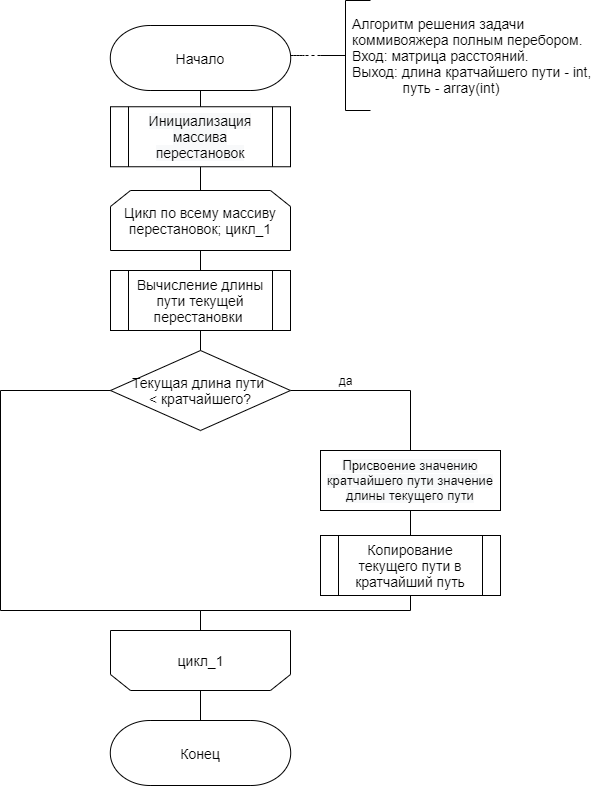
\includegraphics[scale=0.6]{../../../../../../../msys64/home/Лев/bmstu_sem_5_aa/lab_06/report/diagrams/brute_force}
		\caption{Схема алгоритма полного перебора.}
		\label{png:brute_force}
			}
\end{figure}

\newpage
На рисунке \ref{png:ant_1} и  \ref{png:ant_2} представлена схема алгоритма муравьев.
\begin{figure}[H]
	\centering{
		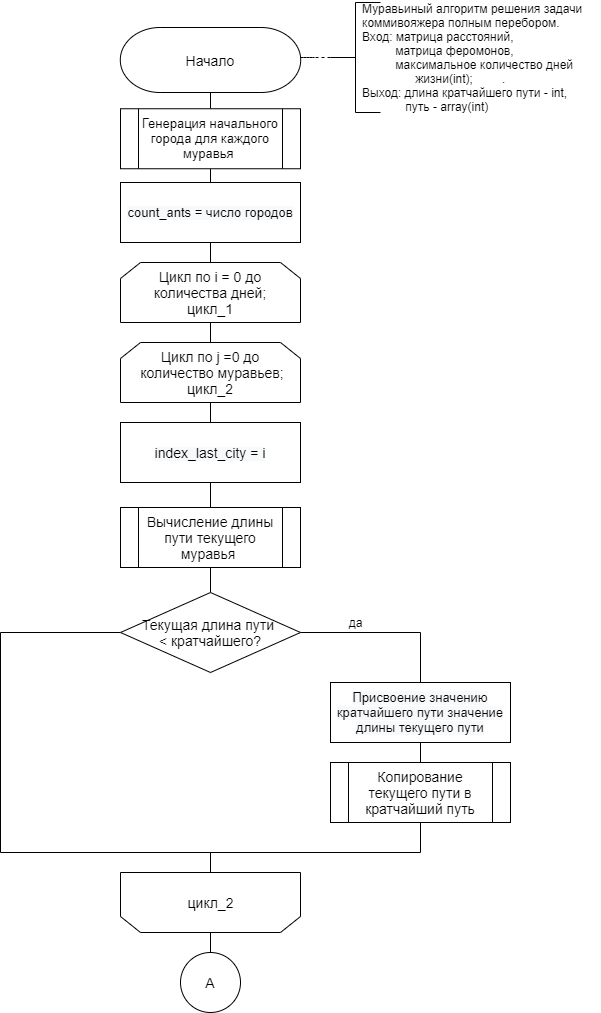
\includegraphics[scale=0.6]{../../../../../../../msys64/home/Лев/bmstu_sem_5_aa/lab_06/report/diagrams/ant_1}
		\caption{Схема алгоритма муравьев.}
		\label{png:ant_1}
	}
\end{figure}

\begin{figure}[H]
	\centering{
		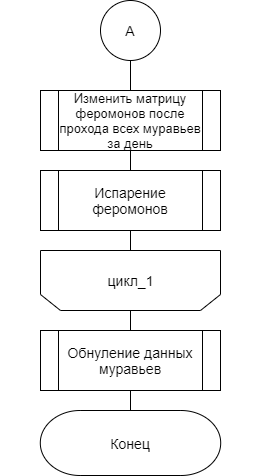
\includegraphics[scale=0.6]{../../../../../../../msys64/home/Лев/bmstu_sem_5_aa/lab_06/report/diagrams/ant_2}
		\caption{Схема алгоритма муравьев.}
		\label{png:ant_2}
	}
\end{figure}

\section{Описание структур данных}
Муравьиная колония представлена структурой данных, которая содержит в себе следующие параметры:
\begin{itemize}
	\item количество дней жизни колонии;
	\item матрица феромонов, которая содержит информацию о количестве феромона в каждом узле;
	\item матрица привлекательности - содержит значение привлекательности маршрута для каждого узла;
	\item мета информация, которая содержит параметры;
	\item массив муравьев.
\end{itemize}

Массив муравьев представляет собой количество муравьев, равное количеству городов, содержит следующие параметры
\begin{itemize}
	\item посещенные города - те города, которые муравей уже посетил;
	\item количество посещенных городов;
	\item длина пройденного пути.
\end{itemize}

Мета информация представляет собой структуру, которая содержит следующие параметры:
\begin{itemize}
	\item коэффициент испарения феромонов;
	\item $\alpha$ - коэффициент жадности;
	\item $\beta$ - коэффициент привлекательности;
	\item Q - коэффициент, который используется для нормирования;
	\item начальное значение феромонов, отличное от нуля.
\end{itemize}

\section{Описание способа тестирования и выделенных классов эквивалентности}
Тестирование программного обеспечения будет выполнено, используя матрицу смежности, а также набор регулируемых параметров. Матрица является симметричной, диагональные элементы равны нулю.

В качестве классов эквивалентности можно выделить стоимость пути между городами: порядка 50-100 и 500-1000 условных единиц.

\section{Описание памяти, используемой алгоритмом}
\subsection{Алгоритм полного перебора}
	Память, необходимая для реализации метода полного перебора, состоит из нескольких параметров, представленных в формуле (\ref{eq:brute_memory}):
	\begin{equation}
		\label{eq:brute_memory}
		M_{brute} = M_{graph} + M_{cities}
	\end{equation}
	где:
	\begin{itemize}
		\item $M_{graph}$ - матрица стоимостей - формула (\ref{eq:graph_brute}):
		\begin{equation}
			\label{eq:graph_brute}
			M_{graph} = size(int) \cdot size(graph\_row) \cdot size(graph\_column);
		\end{equation}
		\item $M_{cities}$ - массив посещенных городов - формула (\ref{eq:cities_brute}):
		\begin{equation}
			\label{eq:cities_brute}
			M_{cities} = size(int) \cdot (count\_cities - 1);
		\end{equation}
	\end{itemize}

\subsection{Муравьиный алгоритм}
	Память, используемая муравьиным алгоритмом, складывается как совокупность следующих параметров, представленных в формуле (\ref{eq:ant_memory}):
	\begin{equation}
		\label{eq:ant_memory}
		M_{colony\_ant} = M_{ants} + M_{max\_days} + M_{meta} + M_{pheromon} + M_{attractiveness}
	\end{equation}
	где:
	\begin{itemize}
		\item $M_{ants}$ - массив муравьев - формула (\ref{eq:ants}):
		\begin{equation}
			\label{eq:ants}
			M_{ants} = count\_ants \cdot (size(int) \cdot count\_cities + size(int) \cdot size(double))
		\end{equation}
	
		\item $M_{max\_days}$ - время жизни колонии - формула (\ref{eq:cities_ant}):
		\begin{equation}
			\label{eq:cities_ant}
			M_{max\_days} = size(int)
		\end{equation}
	
		\item $M_{meta}$ - мета информация - формула (\ref{eq:meta_ant}):
		\begin{equation}
			\label{eq:meta_ant}
			M_{meta} = size(double) \cdot 5
		\end{equation}
	
		\item $M_{attractiveness}$ - матрица феромонов - формула  (\ref{eq:pheromon_memory_ant}):
		\begin{equation}
			\label{eq:pheromon_memory_ant}
			M_{pheromon} = size(double) \cdot size(pheromon\_row) \cdot size(pheromon\_column)
		\end{equation}
	
		\item $M_{attractiveness\_memory\_ant}$ - матрица привлекательности - формула (\ref{eq:attractiveness_memory_ant}):
		\begin{equation}
			\label{eq:attractiveness_memory_ant}
			M_{attractiveness} = size(int) \cdot (count\_cities - 1)
		\end{equation}
	\end{itemize}

\section{Структура программного обеспечения}
В качестве парадигмы было использованы структурное программирование. Программное обеспечение состоит из нескольких модулей:
\begin{itemize}
	\item main - главный модуль, который выполняет вызов функций решения задачи коммивояжера (полный перебор и муравьиный алгоритм);
	\item brute\_force - модуль, содержащий необходимые структуры данных и реализацию метода полного перебора;
	\item ant - модуль, содержащий необходимые структуры данных и реализацию муравьиного алгоритма;
	\item cities - модуль, описывающий необходимые структуры и функции для создания массива городов;
	\item file - модуль, необходимый для считывания данных из файла;
	\item matrix - модуль, содержащий необходимые структуры и функции для создания матриц.
\end{itemize}


\section{Вывод}
Были описаны алгоритмы полного перебора и муравьиным методом. Были описаны структуры данных, необходимые для реализации программного обеспечения. Были выделены классы эквивалентности и описан способ тестирования.